\section{Opgeleverde Producten en Diensten}
In dit hoofdstuk worden de opgeleverde producten en diensten beschreven. Er zal gekeken worden naar nieuwe functionaliteit die toegevoegd is aan zowel de interface als de solver. Daarnaast zullen ook de uitgevoerde diensten, die niet direct een bijdrage leveren aan de functionaliteit van de applicatie, worden toegelicht.

\subsection{Solver}
De nieuwe functionaliteit van de solver kan grotendeels worden onderverdeeld in het chaining algoritme en het vinden van flexibiliteitsintervals. Van deze onderdelen zal in deze paragraaf toegelicht worden hoe deze ge\"implementeerd zijn.

\subsubsection{Chaining}
Een nieuwe functionaliteit die is toegevoegd aan de solver is het chaining algoritme, zoals ge\"introduceerd in paragraaf \ref{subsubsec:chainingoplossing}. Er zijn voor dit algoritme drie verschillende methoden voor het selecteren van een chain ge\"implementeerd, namelijk:

\begin{itemize}
\item Selecteer een willekeurige geschikte chain.
\item Selecteer de eerst gevonden geschikte chain.
\item Gebruik de heuristiek zoals beschreven in paragraaf \ref{subsubsec:chainingoplossing}.
\end{itemize}

Om alle drie methoden te kunnen analyseren, zijn deze allen ge\"implementeerd en kan er gemakkelijk gewisseld worden van methode door een kleine aanpassing in de source code te maken. Uiteindelijk is door middel van de analyse van de flexibiliteit en het aantal voorrangsrelaties dat door de algoritmes toegevoegd wordt besloten om de heuristiek zoals beschreven in paragraaf \ref{subsubsec:chainingoplossing} te gebruiken voor de NedTrain Planner. De analyse van de drie mogelijke heuristieken voor het selecteren van een chain is weergegeven in paragraaf \ref{subsubsec:chaininganalyse}.

Het chaining algoritme is een vereiste voor het berekenen van flexibiliteitsintervallen, omdat dit algoritme ervoor zorgt dat elke oplossing die consistent is met de tijdsconstraints, ook consistent is met de resource constraints. Hierdoor wordt het mogelijk om activiteiten te verschuiven, zonder dat er resource conflicten kunnen ontstaan.

\subsubsection{Linear Programming}
Om voor elke activiteit een flexibiliteitsinterval te vinden moet er, zoals beschreven in paragraaf \ref{subsec:probleemoplossing}, een LP-probleem opgelost worden. Om dit gemakkelijk te kunnen doen, wordt de CLP\footnote{\href{https://projects.coin-or.org/Clp}{projects.coin-or.org/Clp}} (COIN-OR Linear Programming) open source library gebruikt. Deze library verwacht als input een stelsel van lineaire vergelijkingen en een variabele om te optimaliseren en geeft als output de geoptimaliseerde waarde en voor elke variabele de toekenning.

De documentatie van CLP is helaas niet heel erg uitgebreid, maar het is desondanks toch gelukt om het LP-probleem door CLP te laten oplossen. Er moet hiervoor een instantie van de klasse \texttt{ClpModel} worden opgebouwd door het aanmaken en bepalen van variabelen en limieten. Er bestaan verschillende instanties van de \texttt{ClpModel} klasse. Zo is er door ons gebruik gemaakt van de modellen \texttt{ClpSimplex} en \texttt{ClpInterior}. Het grote verschil tussen \texttt{ClpSimplex} en \texttt{ClpInterior} is de manier van oplossen, deze gebruiken namelijk respectievelijk de 'Simplex' en de 'Interior Point' methode. Er is zelf nog een \texttt{Constraints} klasse gemaakt om elke variabele een nummer te geven. De variabelen $t^+_0, t^-_0, \ldots, t^+_n$ en $t^-_n$ krijgen respectievelijk de nummers $0, 1, \ldots, 2 \cdot n$ en $2 \cdot n + 1$. Aan het model moet voor elke variabele een onder- en bovengrens worden gesteld. Er moet een objective functie worden opgegeven en ingesteld dat deze gemaximaliseerd moet worden. Vervolgens kan er aan het model constraints worden toegevoegd. Door een solve methode aan te roepen op het model kan er vervolgens met behulp van de variabele nummers de toegekende waarde van de variabele uit het model worden opgevraagd.

\subsection{Interface}
Er zijn grote en kleine veranderingen aan de interface toegebracht. Kleine veranderingen zijn onder andere het oplossen van bugs die zijn achtergelaten door de vorige projecten die ook aan de NedTrain Planner hebben gewerkt. De grootste veranderingen aan de interface zijn het weergeven van de chains en de flexibiliteitsintervallen. Een voorbeeld van de nieuwe interface kan worden gezien in Figuur \ref{fig:GUIfinal}.

\begin{figure}[H]
\centering
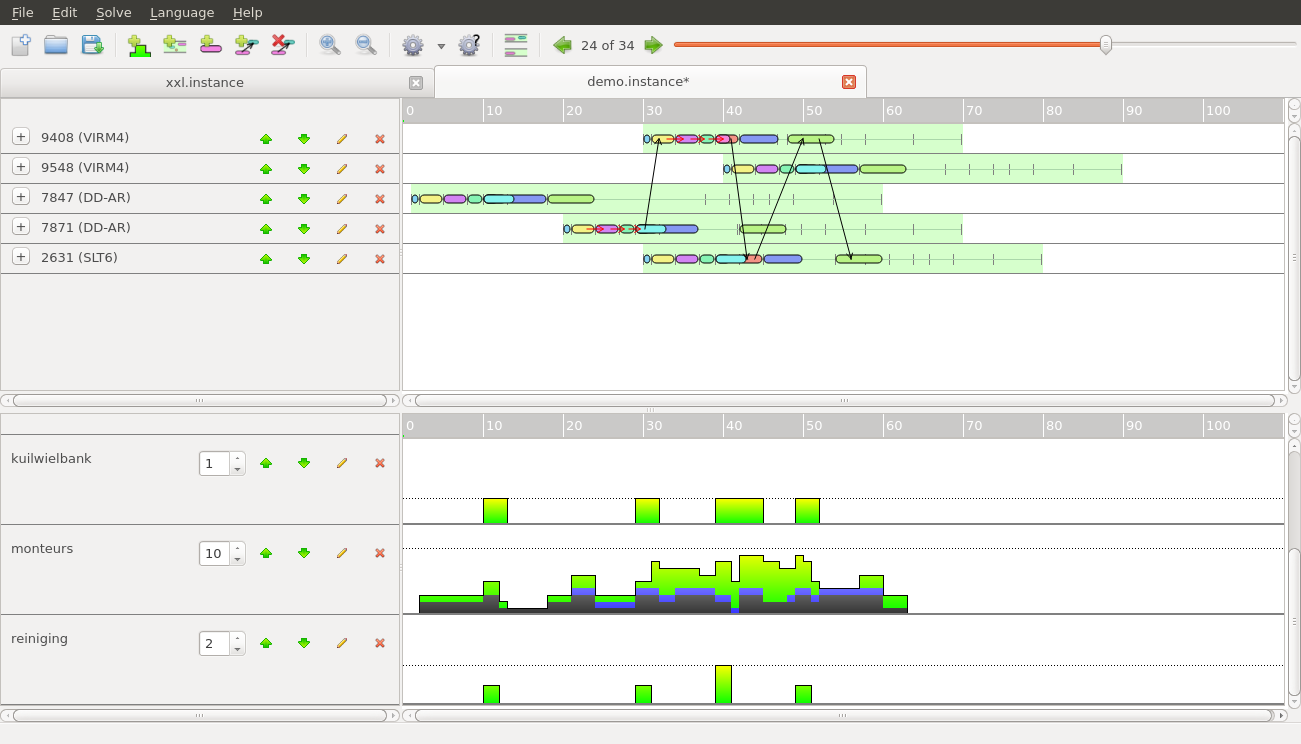
\includegraphics[width=.95\textwidth]{../images/GUIfinal.png}
\caption{De gebruikersinterface.}
\label{fig:GUIfinal}
\end{figure}

In Figuur \ref{fig:GUIfinal} is in de rechterbovenhoek een schuifbalk te zien, waarmee de gebruiker door de verschillende stappen van het proces van de solver kan lopen. Voor elke stap is er een frame opgeslagen waarin de toestand van alle activiteiten staan voor dat moment in het proces van de solver. Als de gebruiker de stappen doorloopt, wordt de corresponderende frame getoond met de opgeslagen informatie in de interface. De volgende frames worden opgeslagen bij het uitvoeren van een solver:
\begin{itemize}
\item Een frame met de begintoestand van de instantie.
\item Voor elke voorrangsrelatie die tijdens het ESTA$^+$ algoritme toegevoegd wordt, een nieuwe frame met daarin alleen de nieuwe voorrangsrelatie en eventuele veranderingen in starttijden van de activiteiten.
\item Een frame zonder voorrangsrelaties, waarin geen resource conflicten meer aanwezig zijn. Op dit moment worden alle eerder toegevoegde voorrangsrelaties verwijderd.
\item Voor elke resource een frame waarin alle bij deze resource horende chains getoond worden. Vervolgens een aparte frame voor elke chain, die elk bij \'e\'en resource unit hoort. Voor lege chains zal er geen frame aangemaakt worden, maar voor chains met maar \'e\'en activiteit wel.
\item Tenslotte een frame waarin voor elke activiteit in het blauw een flexibiliteitsinterval te zien is. Activiteiten worden ook verplaatst, zodat ze zich volledig in het blauwe interval bevinden.
\end{itemize}
Als een solver geen chains en/of flexibiliteitsintervallen berekent, zullen voor deze stappen geen frames worden toegevoegd en zullen alleen de frames van het ESTA$^+$-algoritme getoond worden.

In het frame dat in Figuur \ref{fig:GUIfinal} zichtbaar is, wordt een chain van activiteiten, behorende bij de resource 'monteurs', in het bovenste deelvenster getoond. Hierin zijn de rode pijlen voorrangsrelaties die al in de instantie aanwezig waren en zijn de zwarte pijlen later toegevoegd tijdens het oplossen van de instantie.

Zoals eerder genoemd, worden van een resource eerst alle chains tegelijk getoond op een frame en vervolgens elke chain op een apart frame. Tijdens het \'e\'en voor \'e\'en laten zien van de chains, wordt  het profiel van de gebruikte resources stap voor stap opgebouwd. Op het moment dat er nog geen resources gebruikt worden, is het gehele profiel groen. Bij het tonen van een chain worden alle resource units van een resource die door de activiteiten in deze chain gebruikt worden, in het blauw getoond. Dit betekent dat deze resource units niet meer door andere activiteiten gebruikt kunnen worden. Deze gebruikte resources worden daarom in de daarop volgende frames grijs gekleurd. Zo wordt in elke frame het grijs gekleurde gebied groter, totdat de gehele resource profiel opgevuld is.

\subsubsection{Flexibiliteitsintervallen}
Zoals in Figuur \ref{fig:flex-interval} is te zien, is het ook mogelijk om in de interface het flexibiliteitsinterval van elke activiteit weer te geven. Activiteiten kunnen vrij bewegen binnen het flexibiliteitsinterval zonder dat er conflicten ontstaan met andere activiteiten en zonder dat de starttijden van andere activiteiten veranderen. Als de intervallen worden weergegeven, is het niet mogelijk om de activiteiten buiten het bijbehorende interval te verplaatsen. Ook is het niet mogelijk activiteiten zodanig langer te maken dat ze buiten hun flexibiliteitsinterval vallen. Die twee zaken zijn niet mogelijk, om ervoor te zorgen dat het schema flexibel blijft. Als het weergeven van de flexibiliteitsintervallen wordt uitgezet, kunnen de activiteiten wel verplaatst en vergroot worden buiten het flexibiliteitsinterval.

\begin{figure}[H]
\center
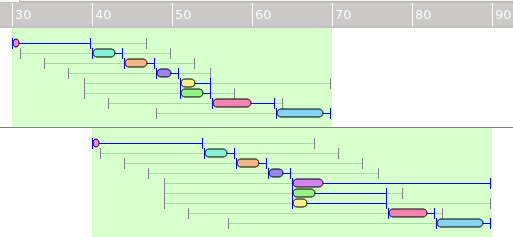
\includegraphics[width=.7\textwidth]{../images/flex-interval.png}
\caption{Flexibiliteitsintervallen}
\label{fig:flex-interval}
\end{figure}

\subsubsection{Rooster}
Naast het resource profiel dat weergegeven kan worden in de onderste helft van de interface \emph{(zie Figuur \ref{fig:GUIfinal})}, is er nu ook een nieuwe manier van het weergeven van de resources die worden gebruikt. Deze nieuwe feature maakt het mogelijk de chains, die worden gegenereerd door het chaining algoritme, op een eenvoudig te begrijpen manier weer te geven. De chains van resource units resulteren in een rooster, dat in de onderste helft van de interface kan worden weergegeven \emph{(zie Figuur \ref{fig:rooster})} met behulp van een nieuwe knop. Vooral als de resource units bijvoorbeeld monteurs, schoonmakers of ander personeel zijn, is deze feature erg handig, omdat de werknemers zelf kunnen zien wie op welk moment aan welke activiteit werkt of pauze heeft. 

\begin{figure}[H]
\center
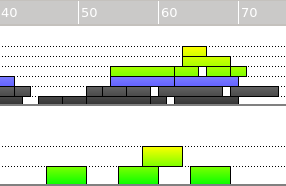
\includegraphics[width=.5\textwidth]{../images/rooster.png}
\caption{Rooster feature}
\label{fig:rooster}
\end{figure}

\subsubsection{Informatie Trein en Activiteit}
Het was al mogelijk om van een activiteit de informatie weer te geven in een klein overzicht. Als er van deze activiteit flexibiliteitsintervallen bekend zijn, worden deze aan het overzicht toegevoegd \emph{(zie Figuur \ref{fig:taak-info})}. Als de instantie nog niet opgelost is of als de instantie is opgelost met een solver die geen flexibiliteitsintervallen ondersteunt, dan worden deze niet in het overzicht weergegeven.  

Nu is er ook een overzicht van informatie over een trein beschikbaar. Als de gebruiker met de rechtermuisknop op de tijdlijn van een trein klikt, maar niet op een activiteit, dan verschijnt er een keuzemenu, waarin de optie 'Treininformatie' gekozen kan worden. Daarmee wordt er een nieuw scherm \emph{(zie Figuur \ref{fig:trein-info})} geopend met daarop informatie zoals het aantal activiteiten en de hoeveelheid resources die minimaal voor deze trein nodig zijn. Vanwege de andere voorwaarden aan het probleem betekent het voldoen aan deze minimumwaarden niet altijd dat de instantie oplosbaar is. Andersom geldt wel dat de instantie nooit oplosbaar is als niet aan de minimale benodigde resources voldaan wordt.

\begin{figure}[H]
\parbox{.45\linewidth}{
    \center
    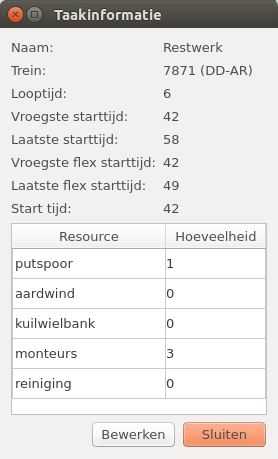
\includegraphics[width=.4\textwidth]{../images/taak-info.png}
    \caption{Taak informatie}
    \label{fig:taak-info}
}\hfill
\parbox{.45\linewidth}{
    \center
    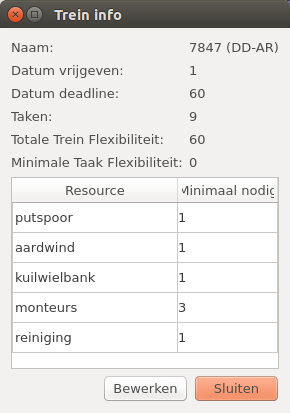
\includegraphics[width=.4\textwidth]{../images/trein-info.png}
    \caption{Trein informatie}
    \label{fig:trein-info}
}
\end{figure}

\subsubsection{Informatie Solver en Oplossing}
Na het oplossen van een instantie door de solver worden de uitkomsten en gegevens van de oplossing gecommuniceerd naar de grafische interface. Zo werd er bijvoorbeeld al doorgegeven hoeveel voorrangsrelaties er aan de instantie zijn toegevoegd door de solver. Nu wordt er ook doorgegeven, als de solver gebruik maakt van flexibiliteitsintervallen, wat de totale flexibiliteit van de oplossing is. Als de gebruiker vervolgens aanpassingen maakt en de instantie vervolgens opnieuw laat oplossen, kan er ook meteen gezien worden wat voor effect dit heeft op het aantal voorrangsrelaties en de totale flexibiliteit. Dit wordt gedaan door het kleuren van de tekst en het geven van de nieuwe en de oude gegevens \emph{(zie Figuur \ref{fig:solver-dialog})}. Een groene kleur van de flexibiliteit tekst geeft aan dat de nieuwe oplossing meer of gelijke flexibiliteit heeft en een rode kleur aangeeft dat de flexibiliteit juist omlaag is gegaan. Hetzelfde geldt voor de tekst van het aantal voorrangsrelaties, waarbij rood aangeeft dat er meer voorrangsrelaties toegevoegd zijn en groen minder of gelijk.

Het is nu ook mogelijk om de tijdsverdeling van de solver na het oplossen te zien. Op deze manier is het meteen duidelijk welk gedeelte van de solver het meest heeft toegedragen aan de totale tijd die de solver nodig had om de instantie op te lossen.

\begin{figure}[H]
    \center
    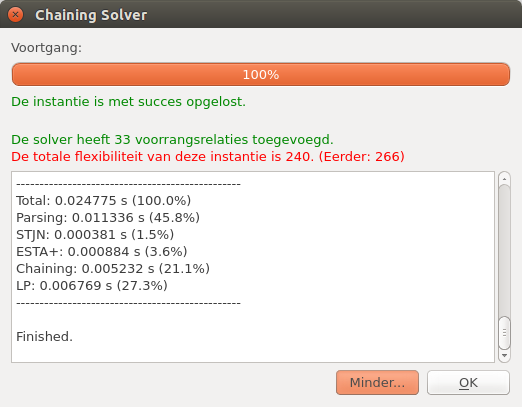
\includegraphics[width=.7\textwidth]{../images/solver-dialog.png}
    \caption{Venster na oplossen van instantie}
    \label{fig:solver-dialog}
\end{figure}

\subsubsection{Gebruiksgemak}
\label{sec:gebruiksgemak}
Om het gebruiksgemak te vergroten, is er een aantal sneltoetsen toegevoegd. Ook is het sluiten van instanties veranderd, want waar eerst instanties gesloten konden worden met een grote rode kruis in de menubalk, is er nu op elke tab van een instantie een klein kruisje geplaatst, waarmee de instantie gesloten kan worden. Dit ontwerp ziet er intu\"itief uit en wordt ook gebruikt door veel bekende browsers zoals Google Chrome en Mozilla FireFox.

Er zijn ook sneltoetsen toegevoegd voor het in- en uitzoomen en voor het horizontaal scrollen. Er kan in- en uitgezoomd worden door de ctrl-toets ingedrukt te houden en het scrollwiel van de muis  te bewegen. Horizontaal scrollen kan in het venster waarin de muis zich op dat moment bevindt door de shift-toets ingedrukt te houden en het scrollwiel van de muis te bewegen. Deze sneltoetsen zijn ingesteld zodat de gebruiker makkelijker door een probleeminstantie kan navigeren, zonder daarvoor steeds zijn muis naar de menubalk te hoeven verplaatsen.

Nog een feature die voor een verbeterd gebruiksgemak moet zorgen bestaat uit de knopjes voor het van plek verwisselen van taken en resources. Dit is vooral handig als er een nieuwe activiteit of resource wordt toegevoegd, want deze wordt altijd onderaan gezet. 

Tijdens het doorlopen van de stappen van het chaining algoritme in de interfaces worden chains opgebouwd voor de resource units van alle resources. Als op een moment chains voor worden aangemaakt voor een bepaalde resource krijgt deze een opvallende kleur. Als dan in de volgende stap een chains worden gemaakt voor een andere resource, dan verspringt het beeld naar die resource en wordt deze ook gehighlight. 

Ten slotte nog een feature die ook prettig is voor gebruikers, maar niet visueel is. Het is mogelijk de applicatie zo te compileren, dat een gebruiker met hetzelfde besturingssysteem de applicatie meteen kan gebruiken, zonder extra software te installeren. Die manier van compileren wordt ook wel \emph{static builden} genoemd. In de \emph{static build} zitten alle afbeeldingen, icoontjes, fonts en externe libraries erbij. Dit maakt het installeren van de applicatie voor de gebruiker stukken gemakkelijker, aagezien er nog al wat afbeeldingen, libraries, ect gebruikt worden in het project. 

\subsection{Codekwaliteit}
Om de codekwaliteit te verbeteren is er een aantal aanpassingen aan de code gemaakt. Deze veranderingen zorgen dus niet voor nieuwe features, maar voor een betere onderhoudbaarheid van de code, zodat ook ontwikkelaars na dit project makkelijk nieuwe features kunnen toevoegen. Zo zijn alle resources (zoals icoontjes, fonts en dergelijke) aan een speciaal bestand, genaamd \texttt{Resources.qrc}, toegevoegd, dat bijhoudt van welke resources de interface gebruik maakt. Door de resources op te sommen in \texttt{Resources.qrc} wordt het in de rest van de code makkelijker hiervan gebruik te maken. Deze verandering is ook nodig voor het static builden van de applicatie, wat wordt besproken in paragraaf \ref{sec:gebruiksgemak}. Ook is het gebruik van \emph{includes} in de code consistenter gemaakt.

In de code van de solver waren veel lange methodes aanwezig, die opgedeeld zijn in een aantal kortere methodes. Ook was er nog typische C code aanwezig, wat niet gebruikelijk is in \cpp\ en soms ook zelfs waarschuwingen gaf tijdens het compileren. In deze gevallen is zo veel mogelijk geprobeerd om de code te laten voldoen aan  \cpp\ conventies. Daarbij zijn het gebruik van een \texttt{boolean} in plaats van een \texttt{integer} en een \texttt{string} in plaats van een \texttt{char*} goede voorbeelden. Ook is er code verwijderd die helemaal niet gebruikt werd.

\subsection{Port naar Windows 7}
Om de toegankelijkheid van de applicatie te vergroten, is er voor gezorgd dat deze ook op het besturingssysteem Windows 7 werkt. Hierbij is het ook nog steeds mogelijk om deze op Unix-based systemen te draaien, zoals Ubuntu. Alle functies van het programma moeten dus zowel op Windows 7 als op Ubuntu correct werken.

\subsection{Upgrade naar Qt 5.2}
De bestaande applicatie was ontwikkeld in versie 4.8 van het Qt framework, maar om de applicatie zo up-to-date mogelijk te houden, is deze geport naar Qt versie 5.2. Hierdoor hoeft een eventuele groep, die de applicatie verder gaat ontwikkelen, niet met een oude versie van het Qt framework te werken. Deze upgrade betekent echter ook dat de applicatie niet meer werkt met Qt 4, maar alleen met versie 5.

\subsection{Behouden van bestaande functionaliteit}
Bij het ontwikkelen van de nieuwe solver is er rekening mee gehouden worden dat alle bestaande functionaliteit behouden blijft. De interface moet dus blijven werken met de bestaande solver en alle functionaliteiten die in de interface ge\"implementeerd zijn, moeten kunnen functioneren op flexibele schema's. Denk hierbij in het bijzonder aan het kunnen vergrendelen van taken, het kunnen instellen van de flexibiliteit en het kunnen verlagen van de resource capaciteit op bepaalde intervallen.
